\chapter{Gesamtsystem}
% ================ Einstellungen =======================
\thispagestyle{fancy} \rhead{\slshape Gesamtsystem}
% ======================================================



\definecolor{myviolett}{RGB}{212,192,226}
\definecolor{myyellow}{RGB}{255,255,178}
\definecolor{myorange}{RGB}{252,231,218}
\definecolor{mygreen}{RGB}{229,241,221}
\definecolor{myblue}{RGB}{225,237,247}
\definecolor{myred}{RGB}{255,178,178}


Abbildung \ref{Blockschaltbild_Gesamtsystem} zeigt das grobe Gesamtsystem des Dojos. Die einzelnen Kapitel dieses Berichts orientieren sich an den Blöcken und deren Funktion im Gesamtsystem. In Kapitel \textbf{\ref{Software} \nameref{Software}} wird die Computersoftware erklärt, welche verwendet wird, um den Dojo zu konfigurieren. Das Kapitel \textbf{\ref{Energieversorgung} \nameref{Energieversorgung}} befasst sich mit dem Akku, der Lade -schaltung und Überwachung, sowie der Spannungsversorgung. Im Kapitel \textbf{\ref{USB} \nameref{USB}} wird erläutert, wie über die USB-Schnittstelle mit dem Mikrocontroller kommuniziert wird und wie Audiofiles auf die SD-Karte übertragen werden. Das Kapitel \textbf{\ref{Audioausgabe} \nameref{Audioausgabe}} behandelt die Verarbeitung und Ausgabe der Audiofiles. Das nächste Kapitel \textbf{\ref{Bluetooth} \nameref{Bluetooth}} befasst sich mit dem Bluetooth. Das heisst, mit den Beacons zur Erkennung der Kunstobjekte und dem Bluetoothmodul im Dojo für den Empfang. Wie die Firmware als Gesamtsystem funktioniert, erfährt man in Kapitel \textbf{\ref{Firmware} \nameref{Firmware}} detailliert. Die Validierung der einzelnen Blöcke wird im jeweiligen Kapitel abgehandelt.

\begin{figure}[h]
	\centering
	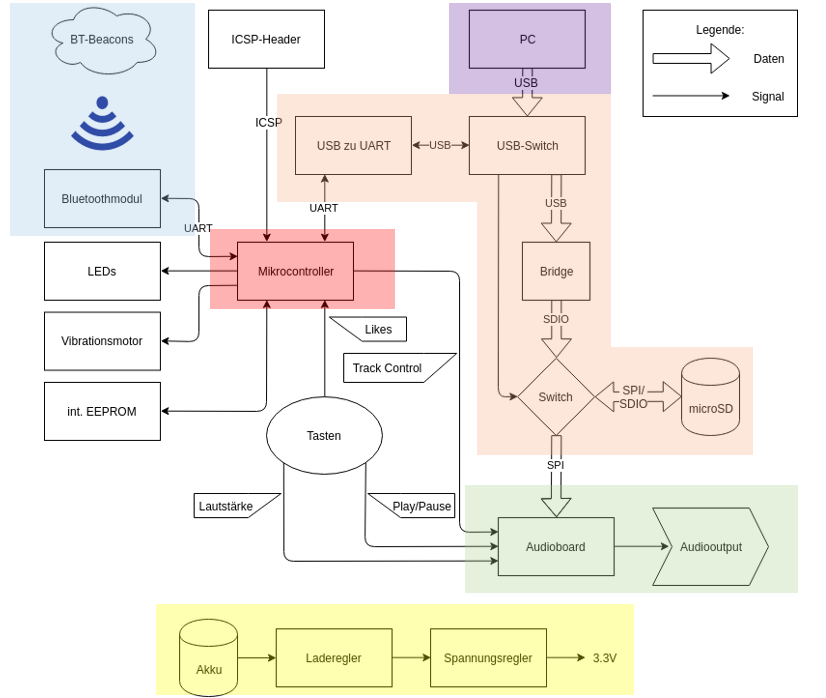
\includegraphics[width=14cm]{Bilder/Gesamtsystem.png}
	\caption{Blockschaltbild Gesamtsystem}
	\label{Blockschaltbild_Gesamtsystem}
\end{figure}

\begin{table}[h]
	\centering
	\begin{tabular}{|c|c|c|c|c|c|} 
		\cellcolor{myviolett}Software & \cellcolor{myyellow}Energieversorgung & \cellcolor{myorange}USB & \cellcolor{mygreen}Audioausgabe & \cellcolor{myblue}Bluetooth & \cellcolor{myred}Firmware \\ 
	\end{tabular} 
	\caption{Legende Gesamtsystem}
	\label{legend_gesamtsystem}
\end{table}
